\subsection{\bf RQ4. Overlapping Analysis}
\label{sec:overlap}

{\footnotesize{
\definecolor{mygray}{gray}{.9}
\begin{table}[t]
  \caption{RQ4. Overlapping Analysis. The number in gray: the unique bugs that a model fixed and the other missed.}
%    \%: \% of the bugs fixed by a tool and missed by the other.}
  \vspace{-9pt}
	\begin{center}
		\renewcommand{\arraystretch}{1}
		\begin{tabular}{p{1cm}<{\centering}|p{0.9cm}<{\centering}|p{1cm}<{\centering}|p{0.7cm}<{\centering}|p{0.9cm}<{\centering}|p{0.8cm}<{\centering}|p{0.7cm}<{\centering}}\hline
			Tool &\multicolumn{3}{c|}{Bugs.jar (1,158 Bugs)}&\multicolumn{3}{c}{BigFix (2,176 Bugs)}\\
			\hline
			{\bf CODIT}             & CODIT   & Overlap   & \tool  & CODIT   & Overlap   & {\tool} \\
			\hline
			Fixed \#     & \cellcolor{mygray} 6  & 80   & \cellcolor{mygray} 91  & \cellcolor{mygray} 13 &  157  & \cellcolor{mygray} 165 \\
%			(\%)            & 6.8\%   &    & 53.4\%  & 7.7\%   &    & 51.4\% \\
			\hline
			{\bf Tufano'19}             & Tufano'19   & Overlap   & \tool  & Tufano'19   & Overlap   & \tool \\
			\hline
			Fixed \#     & \cellcolor{mygray} 5  &  71  & \cellcolor{mygray} 101 & \cellcolor{mygray}4 & 85   & \cellcolor{mygray}237 \\
%			(\%)            &  6.2\%  &    &  58.8\% &  4.9\%  &    & 73.6\% \\
			\hline
			{\bf Seq.R}             & Seq.R   & Overlap   & \tool  & Seq.R   & Overlap   & \tool \\
			\hline
			Fixed \#     & \cellcolor{mygray} 7  &   95 & \cellcolor{mygray} 76 & \cellcolor{mygray} 23 &  158  & \cellcolor{mygray} 164 \\
%			(\%)            &   6.8\% &    & 44.6\%  &   11.2\% &    & 50.9\% \\
			\hline
			{\bf DLFix} & DLFix   & Overlap   & \tool  & DLFix   & Overlap   & \tool \\
			\hline
			Fixed \#     & \cellcolor{mygray}  19 &  105  & \cellcolor{mygray} 66 & \cellcolor{mygray}35 &  211  & \cellcolor{mygray}111 \\
%			(\%)            &  15.0\%  &    & 38.5\%  &  14.2\%  &    &  34.5\%\\
			\hline
			{\bf CoCoNuT}             & CoCoNuT   & Overlap   & \tool  & CoCoNuT   & Overlap   & \tool \\
			\hline
			Fixed \#     & \cellcolor{mygray} 20  & 120   & \cellcolor{mygray} 51 & \cellcolor{mygray}44 &  226  & \cellcolor{mygray} 96\\
%			(\%)            &  14.0\%  &    &  29.7\% &  16.1\%  &    & 29.7\% \\
			\hline
			{\bf CURE}             & CURE   & Overlap   & \tool  & CURE   & Overlap   & \tool \\
			\hline
			Fixed \#     & \cellcolor{mygray} 27  &  126  & \cellcolor{mygray} 45 & \cellcolor{mygray} 50&  233  & \cellcolor{mygray} 89\\
%			(\%)            &  17.4\%  &    & 26.4\%  & 17.7\%   &    &  27.7\%\\
                      	\hline
			{\bf Recoder}             & Recoder   & Overlap   & \tool  & Recoder   & Overlap   & \tool \\
			\hline
			Fixed \#     & \cellcolor{mygray} 40  &  123  & \cellcolor{mygray} 48 & \cellcolor{mygray} 52 &  254  & \cellcolor{mygray} 70\\
%			(\%)            &  24.5\%  &    & 28.1\%  & 17.0\%   &    &  21.6\%\\
			\hline
		\end{tabular}
		\label{RQ3_results}
	\end{center}
\end{table}
}}

%To further study the comparison between {\tool} and the baseline
%models,
%For a comparative study, we performed an overlapping analysis on the
%results.
In Table~\ref{RQ3_results}, each row section corresponds to the
overlapping result between {\tool} and one baseline.
%on Bugs.jar and BigFix.

\subsubsection{{\bf Comparison with CODIT}}

As seen in Table~\ref{RQ3_results}, {\tool} fixed 91 bugs in Bugs.jar
that CODIT missed and CODIT fixed 6 bugs that {\tool} missed. Both fixed the same 80 bugs.
%Among the total number of bugs fixed by either tools in Bugs.jar
%dataset, 53.4\% of them were fixed by {\tool} and missed by CODIT,
%while only 6.8\% of them were fixed by CODIT and missed by {\tool}.
%In BigFix dataset, while {\tool} fixed 165 bugs that CODIT missed,
%it missed only 13 bugs that CODIT fixed.


Figure~\ref{example_codit} shows an example that was correctly fixed
by {\tool}, but missed by CODIT. CODIT fixed it into \code{else}
\code{if(} \code{op)}. CODIT fixed via translation of the buggy AST
sub-tree covering all the edited nodes, without considering the
context.
%. It analyzes the buggy sub-tree that covers all the edited
%nodes {\em without considering the surrounding context} in the method.
%Thus, it did not fix this bug correctly.
In this case, the correct fix is at line 4 by {\tool}: \code{else}
\code{if} \code{(op} \code{instanceof}
\code{ExpressionOperator)}. {\tool} could leverage the surrounding
context at line 7 with `\code{currentOp} \code{instanceof}
\code{ExpressionOperator}' to generate the correct patch at line 4.


%{\color{blue}{1. CODIT only do the prediction and token generation on the buggy sub-tree that covers all edited nodes without considering the other information in the same method. So it cannot catch the information about the variable $ExpressionOperator$ in the method.
%2. Fixing results: \textit{CODIT: else if( op )$ \{$} CDFIX: \textit{else if( op instanceof ExpressionOperator ) $\{$}}}

\begin{figure}[t]
	\centering
	\lstset{
		numbers=left,
		numberstyle= \tiny,
		keywordstyle= \color{blue!70},
		commentstyle= \color{red!50!green!50!blue!50},
		frame=shadowbox,
		rulesepcolor= \color{red!20!green!20!blue!20} ,
		xleftmargin=1.5em,xrightmargin=0em, aboveskip=1em,
		framexleftmargin=1.5em,
		numbersep= 5pt,
		language=Java,
		basicstyle=\scriptsize\ttfamily,
		numberstyle=\scriptsize\ttfamily,
		emphstyle=\bfseries,
		moredelim=**[is][\color{red}]{@}{@},
		escapeinside= {(*@}{@*)}
	}
	\begin{lstlisting}[]
public void visit(LOProject project) throws ... {
  ...
(*@{\color{red}{- else if( op instanceof LOProject ) \{ }}@*)
(*@{\color{cyan}{+ else if( op instanceof ExpressionOperator ) \{ //{\tool}}}@*)
      LogicalExpression expOper = exprOpsMap.get(op);
      ...
      if (currentOp instanceof ExpressionOperator) {
        LogicalExpression exp = exprOpsMap.get(currentOp); ...
      }
// CODIT's incorrect fix at line 3:
// (*@{\color{orange}else if( op)}@*) 
	\end{lstlisting}
        \vspace{-17pt}
	\caption{Comparison with CODIT: An Example}
	\label{example_codit}
\end{figure}

\subsubsection{\bf Comparison with Tufano'19}





As seen in Table~\ref{RQ3_results}, in Bugs.jar, {\tool} can fix 101
bugs that Tufano'19 missed and Tufano'19 fixed only 5 bugs
that {\tool} missed.
%, while both can fix the same 71 bugs.
%Among the total number of bugs fixed by both tools in Bugs.jar
%dataset, 53.4\% of them were fixed by {\tool} and missed by CODIT,
%while only 6\% of them were fixed by CODIT and missed by {\tool}.
%Tien
%In BigFix dataset, while {\tool} can fix 237 bugs that Tufano'19
%missed, it missed only 4 bugs that Tufano'19 can fix. Both {\tool} and
%Tufano'19 can fix the same 85 bugs in BigFix.

Figure~\ref{example_tufano19} shows an example that was fixed by
{\tool}, but missed by Tufano'19. Tufano'19 uses a {\em
  machine translation approach on the entire buggy method}
\code{readFromMemory}.  Because {\em in training, the model did not
  distinguish the buggy statement from the surrounding contex}t,
  %(did not make a clear boundary between them)},
during fixing, the noise from the irrelevant statements in the method
could cause it {\em predict an incorrect statement to be fixed}. In
this example, Tufano'19 incorrectly identified line 2 as a buggy
statement, and fixed it into \code{if(} \code{mMemoryPtr.size}
\code{()} \code{==} \code{0)} \code{return} \code{null;}. The buggy
line 4 was correctly fixed into line 5 by {\tool}. By distinguishing
the context from the fixing changes, {\tool} could learn the type
\code{List} of \code{mContents} from lines 2 and 3 (in which the
method \code{size()} is called on \code{mContents}).

%{\color{blue}{1. Tufano 19' learns and makes prediction only on the method level. In this case, it may fix the wrong position.
%2. Fixing results:
%Tufano 19': \textit{if (mMemoryPtr.size() == 0) return null;} (this fix at line 2)
%CDFIX: \textit{return ((List<Tuple>)mContents).get(mMemoryPtr++);}}}

\begin{figure}[t]
	\centering
	\lstset{
		numbers=left,
		numberstyle= \tiny,
		keywordstyle= \color{blue!70},
		commentstyle= \color{red!50!green!50!blue!50},
		frame=shadowbox,
		rulesepcolor= \color{red!20!green!20!blue!20} ,
		xleftmargin=1.5em,xrightmargin=0em, aboveskip=1em,
		framexleftmargin=1.5em,
		numbersep= 5pt,
		language=Java,
		basicstyle=\scriptsize\ttfamily,
		numberstyle=\scriptsize\ttfamily,
		emphstyle=\bfseries,
		moredelim=**[is][\color{red}]{@}{@},
		escapeinside= {(*@}{@*)}
	}
	\begin{lstlisting}[]
private Tuple readFromMemory() {
  if (mContents.size() == 0) return null;
  if (mMemoryPtr < mContents.size()) {
(*@{\color{red}{-\quad return ((ArrayList<Tuple>)mContents).get(mMemoryPtr++);}}@*)
(*@{\color{cyan}{+\quad return ((List<Tuple>)mContents).get(mMemoryPtr++);}//{\tool} }@*)
  } else {
     return null;
  }
}
// Tufano19's incorrect fix at line 2:
// (*@{\color{orange}if( mMemoryPtr.size () == 0) return null}@*) 
	\end{lstlisting}
        \vspace{-15pt}
	\caption{Comparison with Tufano19': An Example}
	\label{example_tufano19}
\end{figure}
%=============================================================

\subsubsection{\bf Comparison with SequenceR}

As seen in Table~\ref{RQ3_results}, {\tool} fixed 76 bugs in Bugs.jar
that SequenceR missed and SequenceR fixed only 7 bugs that
{\tool} missed.
%, while both can fix the same 95 bugs.
%Among the total number of bugs fixed by both tools in Bugs.jar
%dataset, 53.4\% of them were fixed by {\tool} and missed by CODIT,
%while only 6\% of them were fixed by CODIT and missed by {\tool}.
%In BigFix, among all the bugs fixed by either
%tools, while {\tool} fixed 50.9\% (164 bugs) that SequenceR missed,
%it missed only 11.2\% (23 bugs) that SequenceR fixed.

Figure~\ref{example_3} shows an example that SequenceR missed, but was
fixed correctly by {\tool}. Despite considering the context, {\em
  SequenceR treats source code as a sequence of code tokens}, not
well-suited for structural changes. The fix from line 6 into line 7
involves structural changes to the AST of the statement at line 6
because the order of two operations \code{abs} and \code{\%} is
reversed. In the buggy code, \code{abs} is executed first and then
\code{\%} is next. In the correct code, \code{\%} is executed before
\code{abs}.
%As shown in Figure~\ref{tree-change}, the structure of the
%AST for the statement is changed to reflect the change in that
%order.
However, SequenceR considers the statement as the sequence of tokens,
and it fixed by replacing the token \code{hashCode} with the token
\code{get}. That is, it incorrectly fixed the line 6 into
\code{return} \code{(Math.abs(} \code{keyTuple.} \code{get())}
\code{\%} \code{totalReducers);}.
%Thus, its sequence representation is not well-suited for structural
%changes.

%SequenceR: \textit{return (Math.abs( keyTuple.get()) \% totalReducers);}

\begin{figure}[t]
	\centering
	\lstset{
		numbers=left,
		numberstyle= \tiny,
		keywordstyle= \color{blue!70},
		commentstyle= \color{red!50!green!50!blue!50},
		frame=shadowbox,
		rulesepcolor= \color{red!20!green!20!blue!20} ,
		xleftmargin=1.5em,xrightmargin=0em, aboveskip=1em,
		framexleftmargin=1.5em,
		numbersep= 5pt,
		language=Java,
		basicstyle=\scriptsize\ttfamily,
		numberstyle=\scriptsize\ttfamily,
		emphstyle=\bfseries,
		moredelim=**[is][\color{red}]{@}{@},
		escapeinside= {(*@}{@*)}
	}
	\begin{lstlisting}[]
public int getPartition(...) {
  ...
  indexes = reducerMap.get(keyTuple);
  // if reducerMap does not contain the key, ...
  if (indexes == null) {
(*@{\color{red}{-\quad return (Math.abs(keyTuple.hashCode()) \% tot..);	}}@*)
(*@{\color{cyan}{+\quad return (Math.abs(keyTuple.hashCode() \% tot..));//{\tool}}}@*)
  }
  ...
// SequenceR's incorrect fix at line 6:
// (*@{\color{orange}return (Math.abs( keyTuple. get()) \% totalReducers);}@*)
// CoCoNuT's incorrect fix at line 6:
// (*@{\color{orange}return (Math.abs( keyTuple. hashCode());}@*)
// CURE's incorrect fix at line 6:
// (*@{\color{orange}return (Math.abs( keyTuple. hashCode()) / totalReducers);}@*)
// DLFix's incorrect fix at line 6:
// (*@{\color{orange}return (Math.abs( keyTuple. hashCode()) \% curIndex);}@*)
	\end{lstlisting}
        \vspace{-15pt}
	\caption{Comparison with the Context-aware, DL-based APR baselines: SequenceR, CoCoNuT, CURE, and DLFix}
	\label{example_3}
\end{figure}

%Tien
%\begin{figure}[t]
%	\centering
%	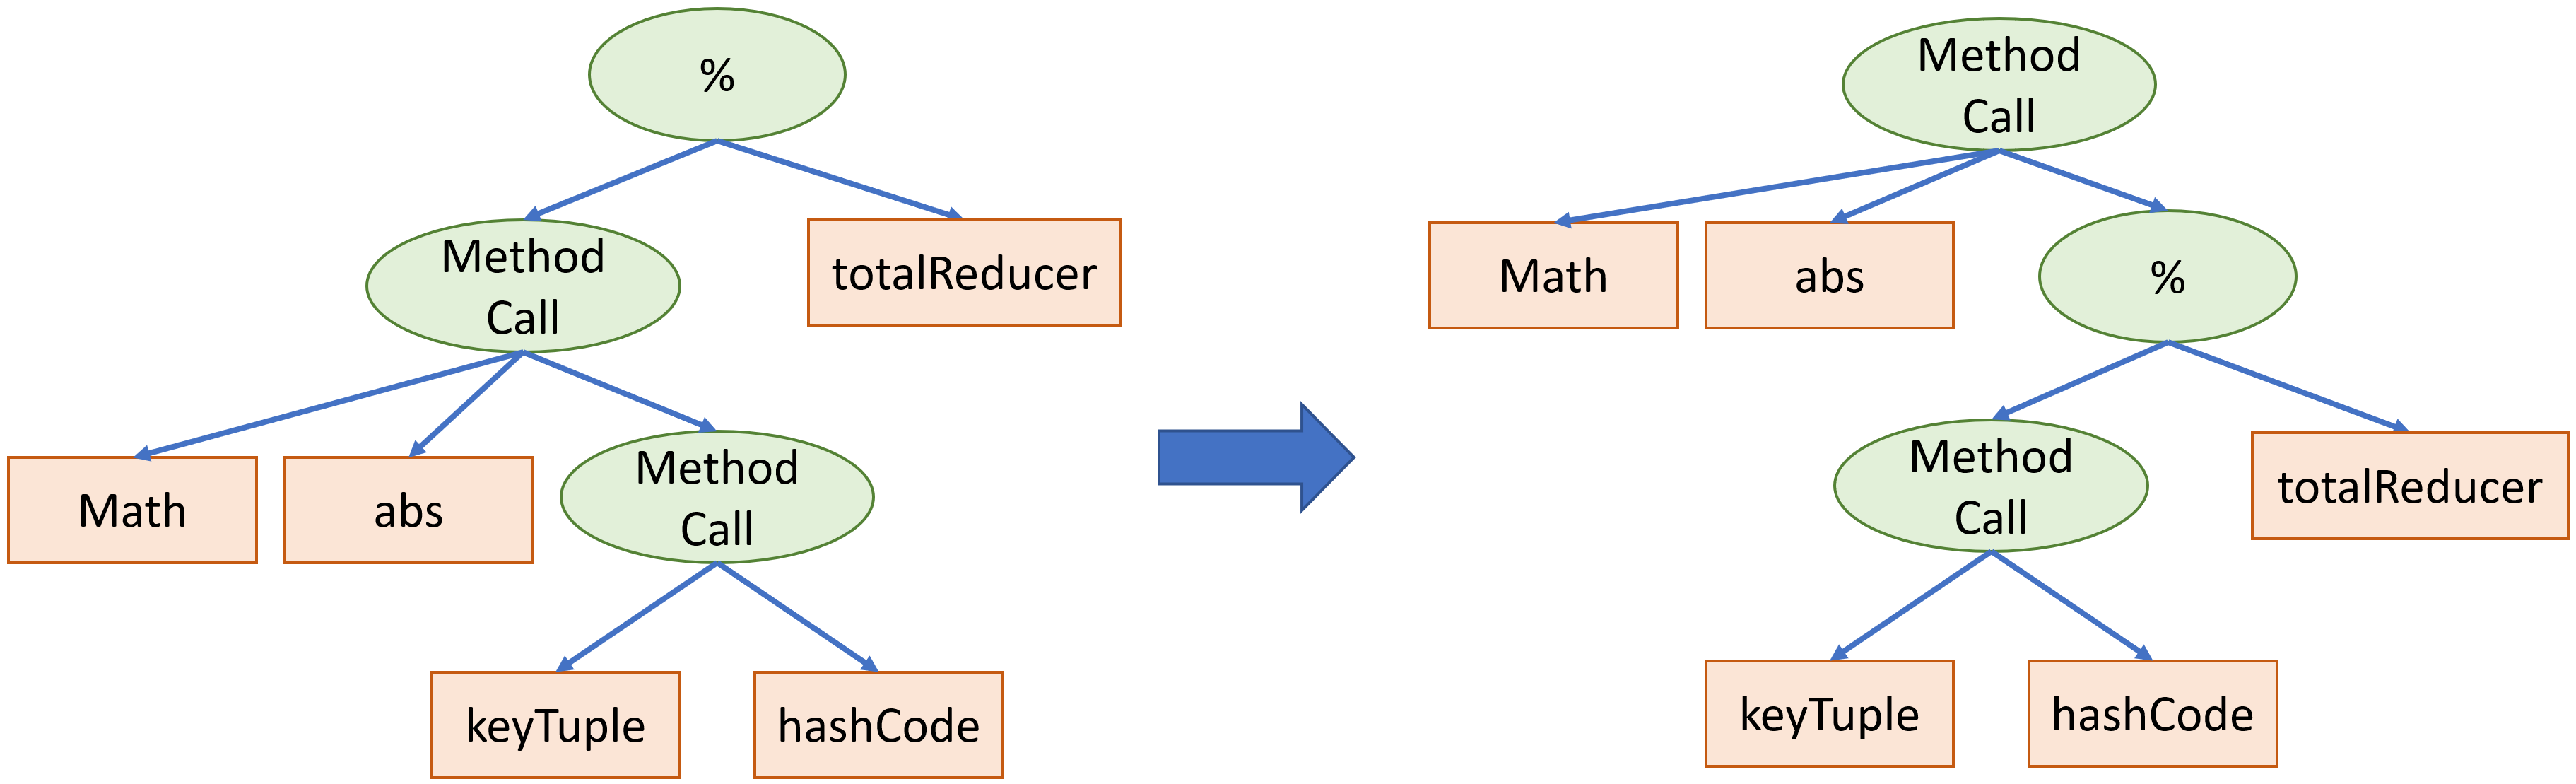
\includegraphics[width=3.1in]{graphs/example_3_v2.png}
%        \vspace{-9pt}
%	\caption{AST Structural Changes for the Fix in Figure~\ref{example_3}}
%	\label{tree-change}
%\end{figure}


\subsubsection{\bf Comparison with CoCoNuT}

As seen in Table~\ref{RQ3_results}, in Bugs\-.jar, {\tool} fixes 51
bugs that CoCoNuT missed and CoCoNuT fixed only 20 bugs that {\tool}
missed.
%, while both fix 120 bugs. Among the total
%number of bugs fixed by either tools in BigFix, 29.7\% of them (96)
%were fixed by {\tool} and missed by CoCoNuT, while only 16.1\% of them (44) were fixed by CoCoNuT and missed by {\tool}.

CoCoNuT did not fix correctly the code in Figure~\ref{example_3}.~It
fixed~line 6 into \code{return (} \code{Math.abs(} \code{keyTuple.}
\code{hashCode} \code{());}. First, CoCoNuT represents source code by
a sequence of tokens, which is {\em not well-suited for this
  structural change}. Second, despite considering the context, CoCoNuT
extracts from the surrounding code the features and feeds them in a
single model for learning to fix.
%
It was shown that dedicating a model for context learning separately
from the transformation learning model can improve APR~\cite{icse20}.
%{\tool} dedicates a model for context learning separately from the
%model for code transformation learning.
With CCL and CTL, {\tool} can learn the structural changes in the AST.

\subsubsection{\bf Comparison with CURE}

As seen in Table~\ref{RQ3_results}, in Bugs.jar, {\tool} can fix 45
bugs that CURE missed and CURE fixed 27 bugs that {\tool} missed.
%while both can fix the same 126 bugs. In BigFix dataset, the number of
%unique bugs that were fixed by {\tool} but missed by CURE is 178\%
%more than the ones that were fixed by CURE but missed by {\tool} (89
%versus 50).

CURE did not fix correctly the example in Figure~\ref{example_3}. It
fixed~line 6 into \code{return (}\code{Math.abs(}
\code{keyTuple.} \code{hashCode())} \code{/} \code{totalReducers);}.
That is, it just replaced the operator \code{\%} with \code{/}.
Compared to CoCoNuT, CURE also represents source code as a sequence of
tokens, thus, is {\em not well-suited to learn the structural changes} for
the fix in this example. CURE is code-aware,
%however, similar to CoCoNuT, it still encodes
and extracts the code-aware features from the context and feeds them
into a single model.
%{\tool} treats context learning with the CCL model separately from
%transformation learning with the CTL model.
%Dual-task learning helps propagate the impact of CCL and CTL
%models on each other.

\subsubsection{\bf Comparison with DLFix}

As seen in Table~\ref{RQ3_results}, in Bugs.jar, {\tool} can fix 66
bugs that DLFix missed and DLFix fixed 19 bugs that {\tool}
missed.
%, while both can fix the same 105 bugs. Among the total
%number of bugs fixed by both tools in BigFix dataset, 34.5\% of them
%were fixed by {\tool} and missed by DLFix, while only 14.2\% of them
%were fixed by DLFix and missed by {\tool}.

DLFix did not fix correctly the buggy code in
Figure~\ref{example_3}. It fixed~the line 6 into \code{return
  (}\code{Math.abs(} \code{keyTuple.} \code{hashCode())} \code{\%}
\code{curIndex);}. Despite that DLFix has separate tree-based models
(handling structural changes) for CCL and CTL,
%for context learning and transformation learning,
it follows a cascading architecture~between them.
%the two models.
Thus, incorrect context learning affects transformation
learning. In this example, \code{curIndex} was incorrectly used in the
fix.

%In {\tool}, context learning and transformation learning are treated
%as a dual task to propagate the impact on each other.


%{\color{blue}{1. SequenceR, CoCoNut, CURE all using sequence structure to do the code fixing. However, it is hard for them to learn the structure changes in this example. DLFix learns the structure changes, but it does not learn it as well as CDFix.
%2. Fixing results:
%SequenceR: \textit{return (Math.abs( keyTuple.get()) \% totalReducers);}
%CoCoNut: \textit{return (Math.abs( keyTuple.hashCode()));}

%DLFix: \textit{return (Math.abs( keyTuple.hashCode()) \% curIndex);}

%CURE: \textit{return (Math.abs( keyTuple.hashCode()) / totalReducers);}

%CDFIX: \textit{return (Math.abs( keyTuple.hashCode() \% totalReducers));}}}





%Table~\ref{RQ3_results} shows the overlapping analysis of the bugs fixed by {\tool} and the studied baselines. The results show that {\tool} can fix more unique bugs than any compared baseline. For example, {\tool} can fix 89 bugs that cannot be fixed by CURE, while CURE can fix 50 bugs that our {\tool} cannot fix.


%Consolidating results from RQ2 and RQ3, overall, {\tool} can auto-fix more bugs and unique bugs than any studied baselines, indicating that {\tool} is better and complementary to other baselines.

\subsubsection{\bf Comparison with Recoder}

As seen in Table~\ref{RQ3_results}, in Bugs.jar, {\tool} can fix 48
bugs that Recoder missed and Recoder fixed 40 bugs that {\tool}
missed. Recoder is designed for single-hunk bugs, thus missed
those 40 multi-hunk/multi-statement bugs. {\tool} handles
the transformation for each buggy AST subtree, thus, supporting
those bugs.
